
\begin{paracol}{2}
\begin{leftcolumn}
  {\allyFont ally} began and still exists as a work of interactive fiction presented on the web. The project now exists in book form out of some neurotic sense of completeness. Perhaps, were I able to hold my life in my hands --- truly hold it, feel the pages sliding against one another --- I would be able to somehow digest it a little bit better. Perhaps, were I able to hold it in my hands, I would be able to understand it. Perhaps I would be able to move on.

  \begin{ally}
    Is anything so simple?
  \end{ally}
  No.

  That said, the project is still available online for your perusal. It works somewhat differently, containing branching paths rather than the tortured layouts of these pages.

  Perhaps the story will continue there.

  \begin{ally}
    And perhaps not.
  \end{ally}
\end{leftcolumn}
\begin{rightcolumn}
  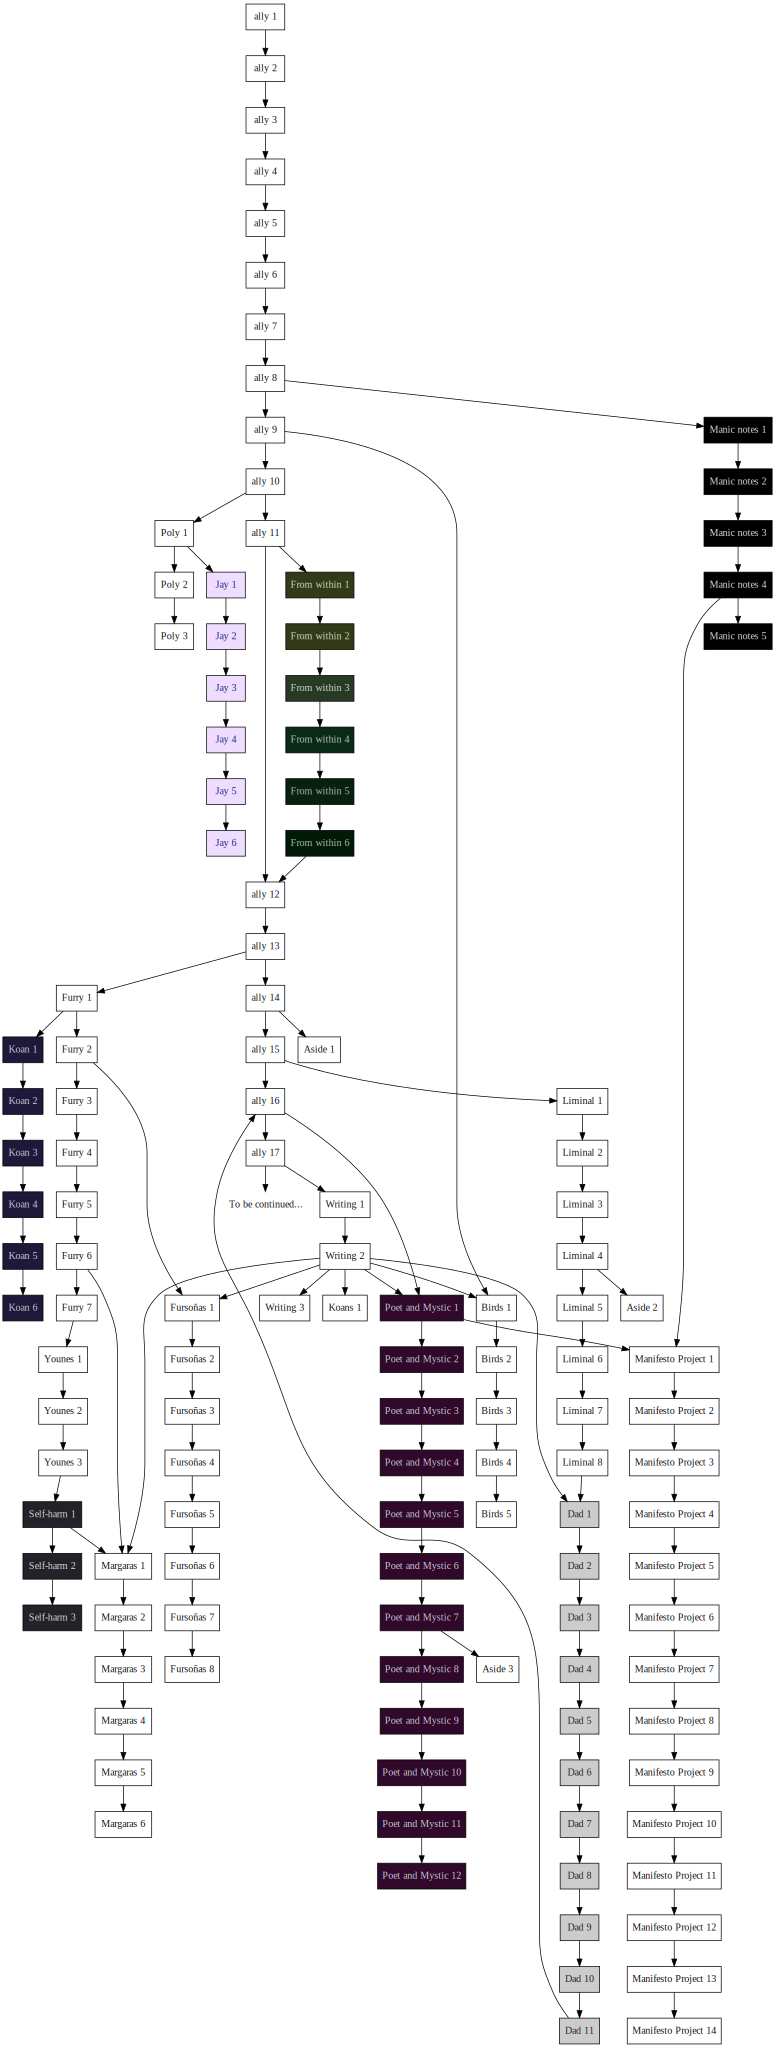
\includegraphics[width=2in]{assets/map.png}
\end{rightcolumn}
\end{paracol}
\newpage

\begin{paracol}{2}
\begin{leftcolumn}
\includegraphics[width=4in]{assets/cadmiumtea--MurderYourDarlings--makyo--G.jpg}

\emph{Murder your darlings} by Julian Norwood

www.patreon.com/cadmiumtea
\end{leftcolumn}
\begin{rightcolumn}
    \null
    \vfill
\noindent Madison Scott-Clary is a transgender author, poet, and programmer. She is also the editor-in-chief of Hybrid Ink, LLC, a small publisher focused on thoughtful fiction, exploratory poetry, and creative non-fiction. She lives in the Pacific Northwest with her cat and two dogs, as well as her husband, who is also a dog.


\begin{center}
    www.makyo.ink

    www.hybrid.ink
\end{center}
\vfill
\end{rightcolumn}
\end{paracol}
